\documentclass{standalone}
\usepackage[T1]{fontenc}
\usepackage{amsmath,amssymb}
\usepackage{pgfplots,pifont}

\begin{document}
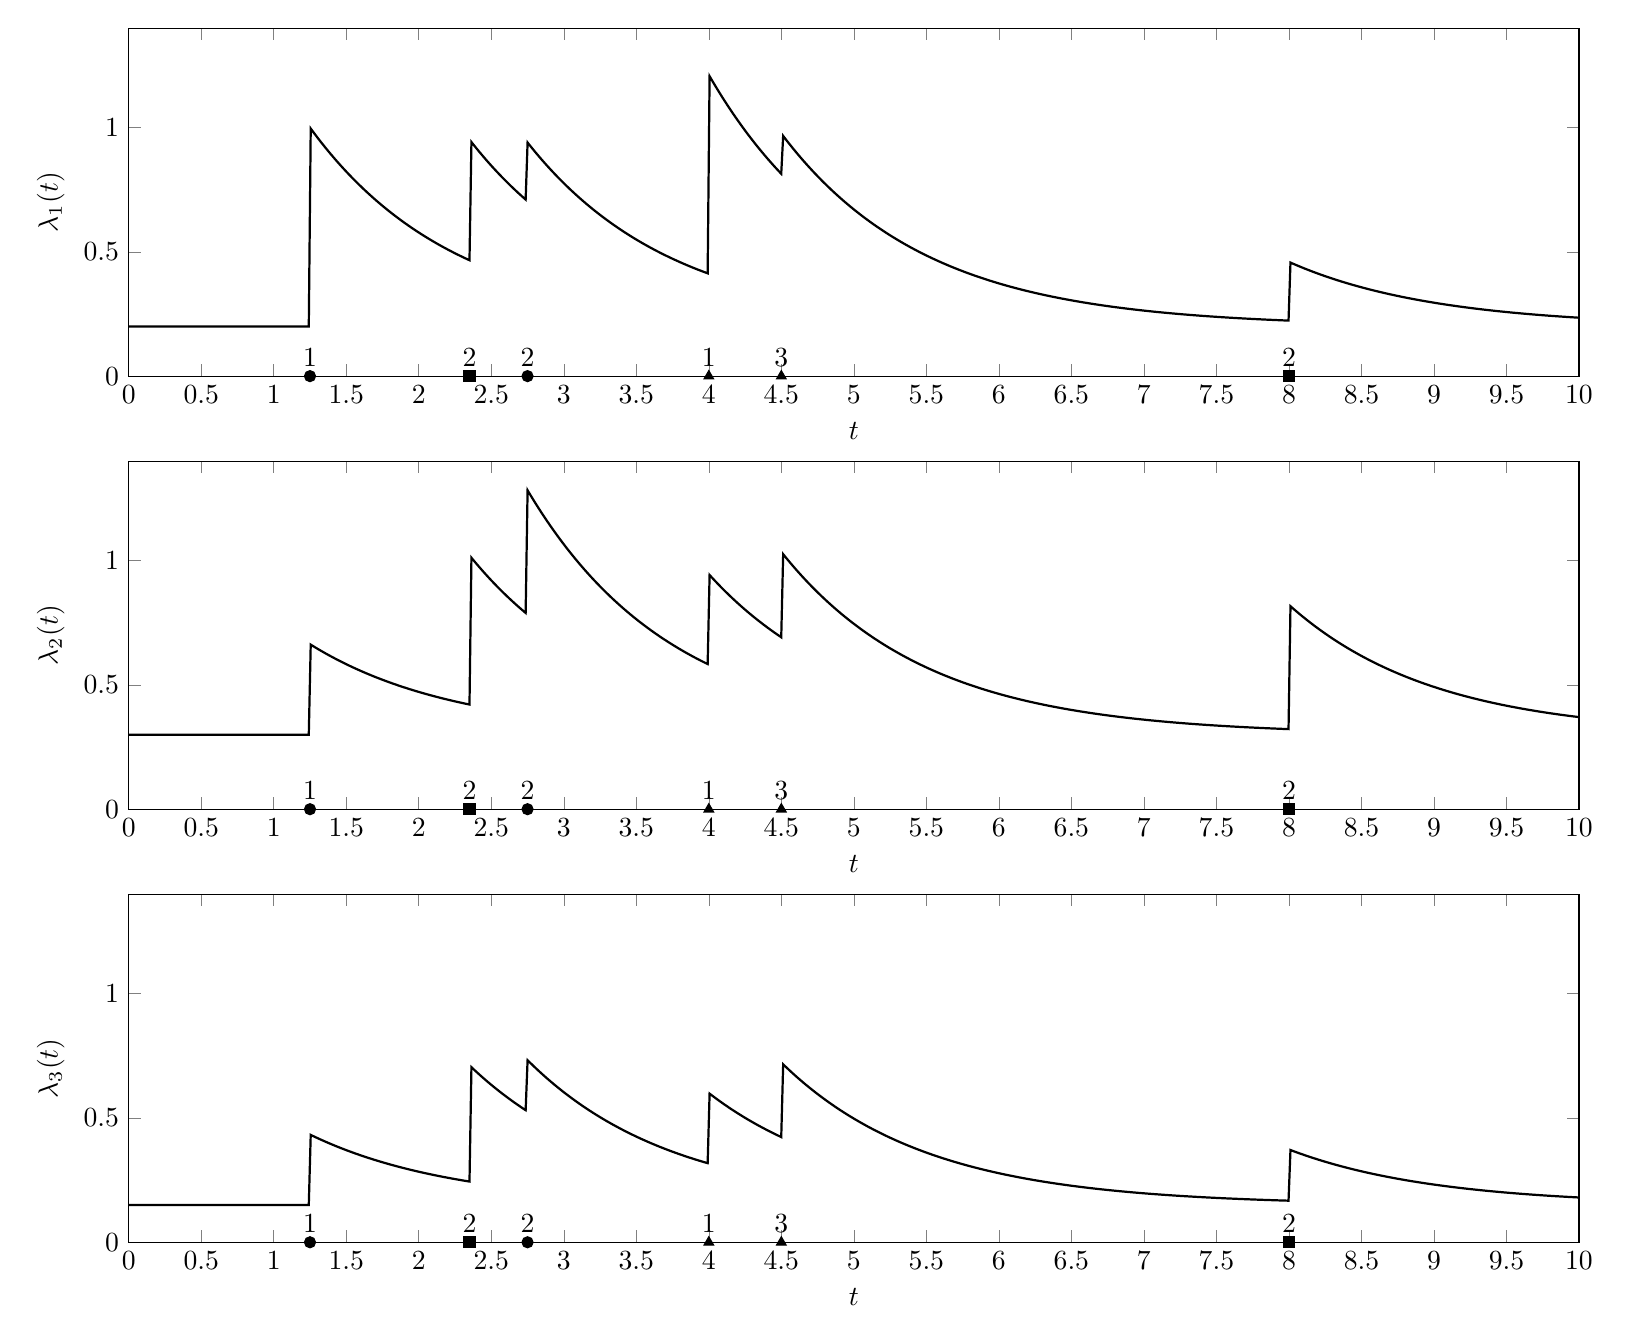
\begin{tikzpicture}


\begin{axis}[
    at={(0,0cm)}, % Adjust the vertical separation
    anchor=north,
    xmin=0,xmax=10,ymin=0,ymax=1.4,xlabel=$t$,ylabel=$\lambda_{1}(t)$,height=6cm,width=20cm, legend cell align={left}]
	
	%% Parameters
	\def\lam{0.2}
	\def\alpha{0.8}
	\def\beta{1}
	\def\theta{1}
	\def\alphap{0.5}
	\def\betap{1}
	\def\thetap{1.5}
	%% Distances
	\def\gammaab{0.5}	
	\def\gammaac{0.75}	
	\def\gammabc{0.25}	
	
	\addplot[domain=0:10, samples=750, style=thick] {(\lam + 
	(x > 1.25 ? \alpha*exp(-\beta*(x-1.25)) : 0) + % Start event 1 - Station 1
	(x > 2.75 ? exp(-\thetap*\gammaab)*\alphap*exp(-\betap*(x-2.75)) : 0) + % End event 1 - Station 2
	(x > 2.35 ? exp(-\theta*\gammaab)*\alpha*exp(-\beta*(x-2.35)) : 0) + % Start event 2 - Station 2
	(x > 4.00 ? \alpha*exp(-\beta*(x-4.0)) : 0) + % Start event 3 - Station 1
	(x > 4.50 ? exp(-\thetap*\gammaac)*\alphap*exp(-\betap*(x-4.5)) : 0) + % End event 3 - Station 3
	(x > 8.00 ? exp(-\thetap*\gammaab)*\alphap*exp(-\betap*(x-8)) : 0)) % End event 2 - Station 2
	};
	
	\addplot[mark=*, nodes near coords={$1$}] coordinates {(1.25,0)};
	\addplot[mark=*, nodes near coords={$2$}] coordinates {(2.75,0)};
	\addplot[mark=square*, nodes near coords={$2$}] coordinates {(2.35,0)};
	\addplot[mark=triangle*, nodes near coords={$1$}] coordinates {(4.0,0)};
	\addplot[mark=triangle*, nodes near coords={$3$}] coordinates {(4.5,0)};
	\addplot[mark=square*, nodes near coords={$2$}] coordinates {(8,0)};

\end{axis}

\begin{axis}[
    at={(0,-5.5cm)}, % Adjust the vertical separation
    anchor=north,
    xmin=0,xmax=10,ymin=0,ymax=1.4,xlabel=$t$,ylabel=$\lambda_{2}(t)$,height=6cm,width=20cm, legend cell align={left}]
	
	%% Parameters
	\def\lam{0.3}
	\def\alpha{0.6}
	\def\beta{1}
	\def\theta{1}
	\def\alphap{0.5}
	\def\betap{1}
	\def\thetap{1.5}
	%% Distances
	\def\gammaab{0.5}	
	\def\gammaac{0.75}	
	\def\gammabc{0.25}	
	
	\addplot[domain=0:10, samples=750, style=thick] {(\lam + 
	(x > 1.25 ? exp(-\theta*\gammaab)*\alpha*exp(-\beta*(x-1.25)) : 0) + % Start event 1 - Station 1
	(x > 2.75 ? \alphap*exp(-\betap*(x-2.75)) : 0) + % End event 1 - Station 2
	(x > 2.35 ? \alpha*exp(-\beta*(x-2.35)) : 0) + % Start event 2 - Station 2
	(x > 4.00 ? exp(-\theta*\gammaab)*\alpha*exp(-\beta*(x-4.0)) : 0) + % Start event 3 - Station 1
	(x > 4.50 ? exp(-\thetap*\gammabc)*\alphap*exp(-\betap*(x-4.5)) : 0) + % End event 3 - Station 3
	(x > 8.00 ? \alphap*exp(-\betap*(x-8)) : 0)) % End event 2 - Station 2
	};
	
	\addplot[mark=*, nodes near coords={$1$}] coordinates {(1.25,0)};
	\addplot[mark=*, nodes near coords={$2$}] coordinates {(2.75,0)};
	\addplot[mark=square*, nodes near coords={$2$}] coordinates {(2.35,0)};
	\addplot[mark=triangle*, nodes near coords={$1$}] coordinates {(4.0,0)};
	\addplot[mark=triangle*, nodes near coords={$3$}] coordinates {(4.5,0)};
	\addplot[mark=square*, nodes near coords={$2$}] coordinates {(8,0)};

\end{axis}

\begin{axis}[
    at={(0,-11cm)}, % Adjust the vertical separation
    anchor=north,
    xmin=0,xmax=10,ymin=0,ymax=1.4,xlabel=$t$,ylabel=$\lambda_{3}(t)$,height=6cm,width=20cm, legend cell align={left}]
	
	%% Parameters
	\def\lam{0.15}
	\def\alpha{0.6}
	\def\beta{1}
	\def\theta{1}
	\def\alphap{0.3}
	\def\betap{1}
	\def\thetap{1.5}
	%% Distances
	\def\gammaab{0.5}	
	\def\gammaac{0.75}	
	\def\gammabc{0.25}	
	
	\addplot[domain=0:10, samples=750, style=thick] {(\lam + 
	(x > 1.25 ? exp(-\theta*\gammaac)*\alpha*exp(-\beta*(x-1.25)) : 0) + % Start event 1 - Station 1
	(x > 2.75 ? exp(-\thetap*\gammabc)*\alphap*exp(-\betap*(x-2.75)) : 0) + % End event 1 - Station 2
	(x > 2.35 ? exp(-\theta*\gammabc)*\alpha*exp(-\beta*(x-2.35)) : 0) + % Start event 2 - Station 2
	(x > 4.00 ? exp(-\theta*\gammaac)*\alpha*exp(-\beta*(x-4.0)) : 0) + % Start event 3 - Station 1
	(x > 4.50 ? \alphap*exp(-\betap*(x-4.5)) : 0) + % End event 3 - Station 3
	(x > 8.00 ? exp(-\thetap*\gammabc)*\alphap*exp(-\betap*(x-8)) : 0)) % End event 2 - Station 2
	};
	
	\addplot[mark=*, nodes near coords={$1$}] coordinates {(1.25,0)};
	\addplot[mark=*, nodes near coords={$2$}] coordinates {(2.75,0)};
	\addplot[mark=square*, nodes near coords={$2$}] coordinates {(2.35,0)};
	\addplot[mark=triangle*, nodes near coords={$1$}] coordinates {(4.0,0)};
	\addplot[mark=triangle*, nodes near coords={$3$}] coordinates {(4.5,0)};
	\addplot[mark=square*, nodes near coords={$2$}] coordinates {(8,0)};

\end{axis}

\end{tikzpicture}
\end{document}
